\documentclass[12pt]{article}
 
\usepackage[margin=1in]{geometry} 
\usepackage{amsmath,amsthm,amssymb,bm}
\usepackage{graphicx}
\usepackage[ruled]{algorithm2e} % Algorithms 
\usepackage[caption = false]{subfig}
 
\begin{document}
  
\title{Task 3. Reinforcement Learning}
\author{Garoe Dorta-Perez\\
CM50245: Computer Animation and Games II}
 
\maketitle
 
\section{Introduction}

\section{A* path finding}

The A*\cite{Hart1968} algorithm can find the shortest paths in a graph, searching within a minimal number of nodes for a given heuristic.
It works under the assumption that the distance heuristic will never overestimate the cost of the path, and the path cost will not decrease as we travel through it.
In a maze world, where the movement possibilities are north, south, east and west, with fixed positive costs, using the Manhattan distance for the real path cost, and the euclidean distance to compute the heuristic cost will fit the aforementioned assumptions.

In Algorithm \ref{alg:A_start}, an overview of a pseudocode implementation of the A* is shown.
As stated in the previous paragraph, graph.cost() and heuristic() returns the Manhattan and the euclidean distance between two nodes, respectively. 
The key idea, is that promising directions, those with a lower heuristic cost will be explored first, thus the exploration favours directions that move towards the goal.
Moreover, since the heuristic will always underestimate the cost, if a path looks good from an heuristic point of view, yet it is actually poor choice, when the path is explored, its cost will lower its priority in the frontier, so the search will continue at the next best guess.
An example output with a small labyrinth where a path is successfully found is shown in Figure \ref{fig:A_start}.

\begin{algorithm}[htbp!] \label{alg:A_start}
	\caption{A*}
	\KwData{$goal$ goal position, $start$ start position, $graph$ graph with the tiles in the map.}
	\KwResult{$path$ path from $start$ to $goal$, $cost$ total cost of the path.}
	
	frontier = PriorityQueue(start, 0)\;
	came\_from[start] = None\;
	cost\_so\_far[start] = 0\;

	\While{not frontier.empty()}{
		current = frontier.get()\;

		\If{current == goal}{
		  break\;
		}
		\For{next in graph.neighbors(current)}{
		  new\_cost = cost\_so\_far[current] + graph.cost(current, next)\;
		  \If{next not in cost\_so\_far or \text{new}\_cost \textless cost\_so\_far[next]}{
			 cost\_so\_far[next] = new\_cost\;
			 priority = new\_cost + heuristic(goal, next)\;
			 frontier.put(next, priority)\;
			 came\_from[next] = current\;
			 }
		}
	}
	$path$ = getPath(came\_from)\;
	$goal$ = cost\_so\_far[current]\;
\end{algorithm}

\begin{figure}[htbp!]
\centering
\begin{minipage}[t]{0.3\linewidth}
	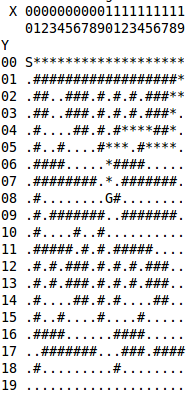
\includegraphics[scale=0.6]{images/a_star_res1}
	\caption{Path finding example, $S$ is the start position, $G$ is the goal position, $*$ are the path points, $.$ are empty spaces and \# are walls.}
	\label{fig:A_start}
\end{minipage}
\quad
\begin{minipage}[t]{0.45\linewidth}
	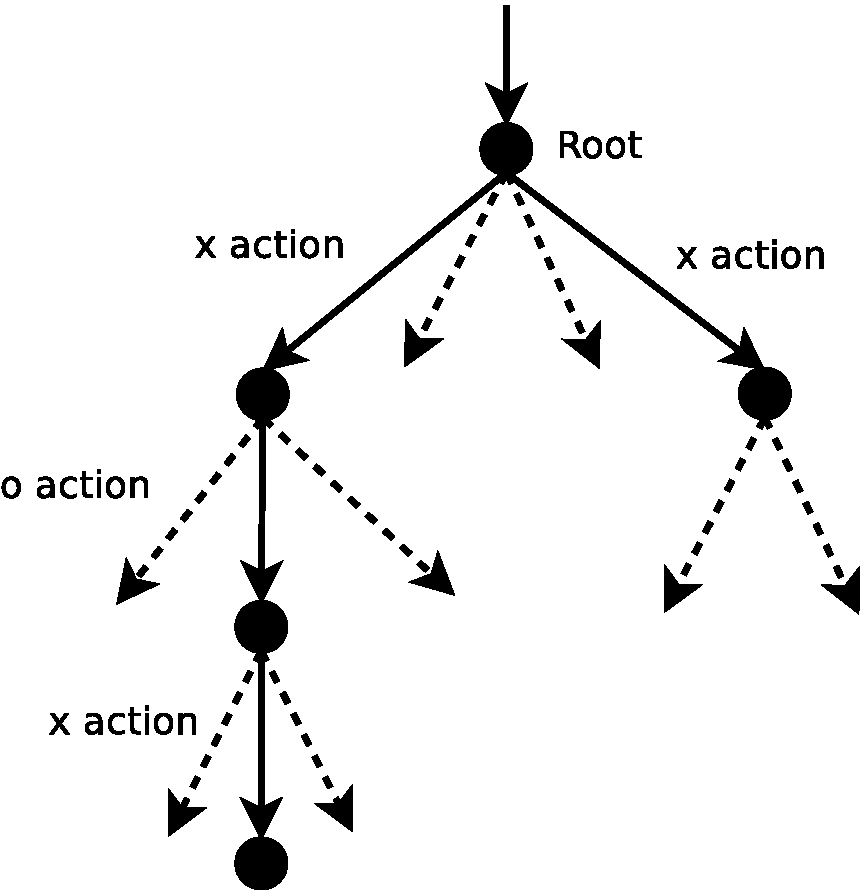
\includegraphics[scale=0.4]{images/ttt_tree}
	\caption{Noughts and crosses tree state.}
	\label{fig:ttt_tree}
\end{minipage}
\end{figure}

\section{TD learning in noughts and crosses}
\label{sec:td_ttt}

Temporal-difference learning\cite{Sutton1998} is a reinforcement learning technique used when a problem can be modelled as a Markov decision process, the world is modelled as a chain of \emph{states}, where an \emph{agent} can take \emph{actions}, each of which are associated with a new state and a \emph{reward}.
The objective is to maximize the rewards that the agents gets, and by doing so, taking the optimal actions in the given world.
However, since the system is an online learner, there is a trade-off between \emph{exploitation}, where the agent takes actions that lead to the highest expected reward, and \emph{exploration}, where the agent takes suboptimal actions to acquire information from unexplored states.

Each state $s$ has a value $V(s)$ associated to it; the agent will choose either, a greedy exploitation action by performing an action $a$ such that the next state $s'$  will be $\max V(s_{t + 1})$, or a exploration action $a$ such that the next state $s'$  will be chosen randomly.
When an end state is reached, the values for each state where a greedy action was taken, will be updated by a backtracking mechanism $V(s) = V(s) + \alpha \left[ V(s') - V(s) \right]$, where $\alpha$ is the learning rate.
In order to have a policy update which asymptotically guarantees convergence, it is a necessary condition for $\alpha$ to decrease its value over time.

Nought and crosses can be modelled as a Markov decision process, given that each board state characterizes the sum of the moves that lead to such state.
The agent is one of the players, a state is a given configuration of a board and rewards are delivered when a game ends.
The agent will receive a high positive reward when they win, a negative reward when they loose and a small positive reward for drawing.

In the implementation, the state space will be modelled in a tree as shown in Figure \ref{fig:ttt_tree}.
On the root of the tree, we have empty board, the children are the 9 possible plays for the crosses player, who will always be the first to play.
Its children the next possible moves for the noughts player and so on.

To test our system, the agent would play a fixed number of games against an AI with fixed moves initialized randomly.
In Figures \ref{fig:ttt_eps_0_2}, \ref{fig:ttt_eps_0_4} and \ref{fig:ttt_eps_0_6}, each curve represents the value for placing a cross in each of the 9 available positions in a new game as the first move.
The reward for winning, drawing and loosing a game was set to 10, 1 and -1 respectively.
Since the adversary of the agent is deterministic, a first move that leads to a winning combination is quickly discovered, and its value is therefore increased. 
In Figure \ref{fig:tttExpectedGain}, a comparison of mean gains after playing a fixed number of games is shown; higher exploitation rates entail increased mean rewards, as expected in a simple game with a deterministic opponent.

\begin{figure}[htbp!]
\centering
\begin{minipage}[t]{0.45\linewidth}
	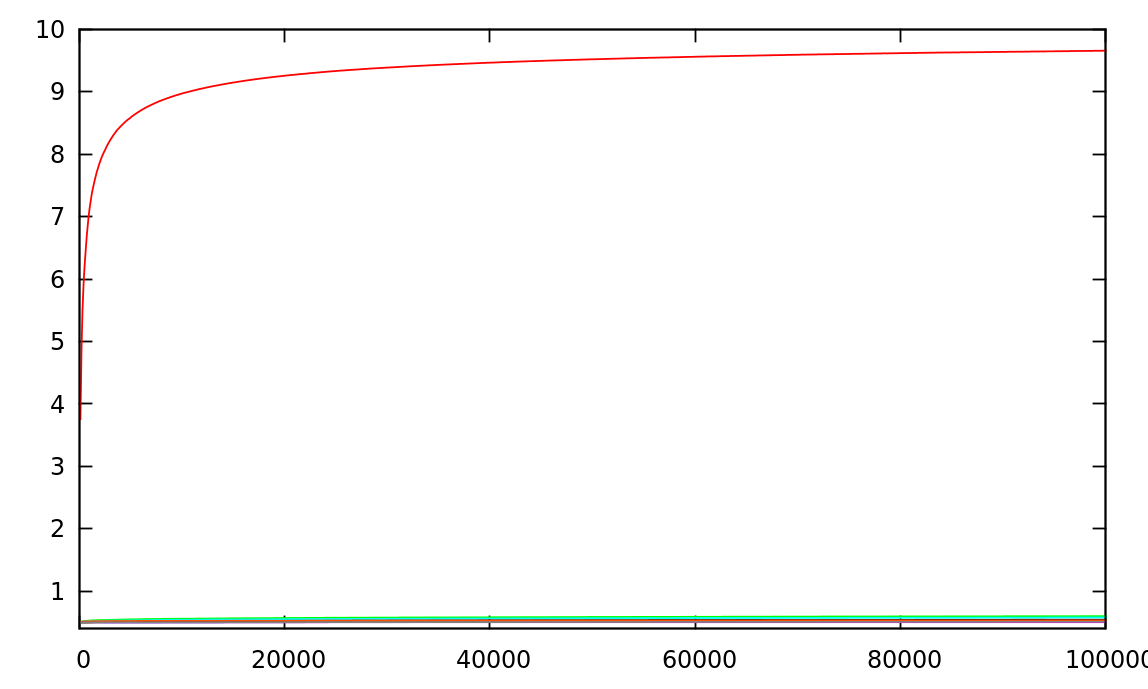
\includegraphics[scale=0.25]{images/ttt_eps_0_2}
	\caption{Values for the first movement for noughts and crosses with 20\% exploration rate after 100000 games.}
	\label{fig:ttt_eps_0_2}
\end{minipage}
\quad
\begin{minipage}[t]{0.45\linewidth}
	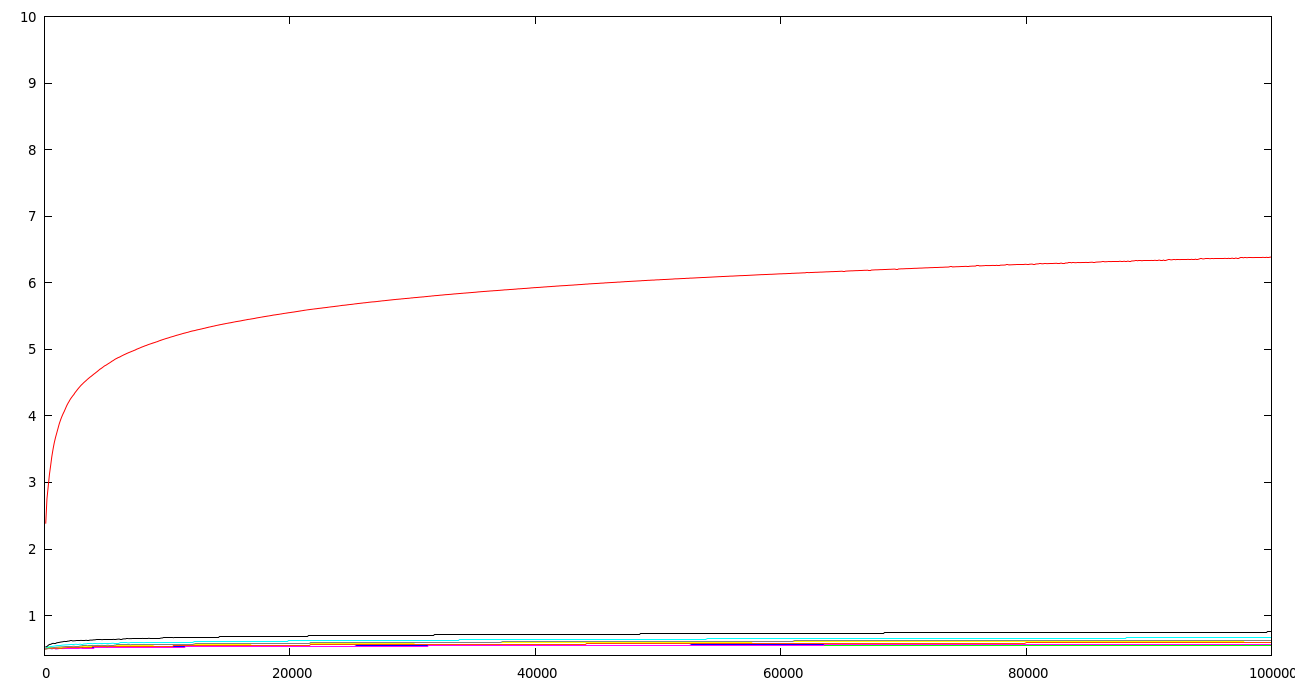
\includegraphics[scale=0.23]{images/ttt_eps_0_4}
	\caption{Values for the first movement for noughts and crosses with 40\% exploration rate after 100000 games.}
	\label{fig:ttt_eps_0_4}
\end{minipage}
\\
\begin{minipage}[t]{0.5\linewidth}
	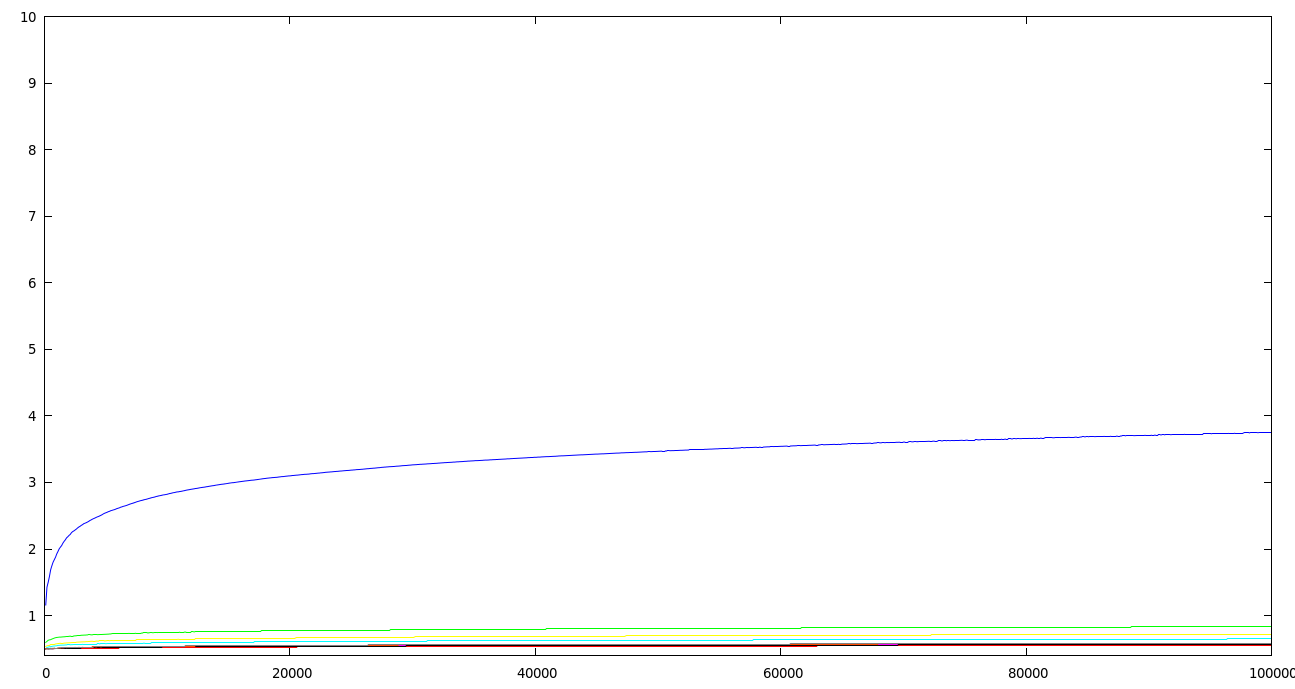
\includegraphics[scale=0.23]{images/ttt_eps_0_6}
	\caption{Values for the first movement for noughts and crosses with 60\% exploration rate after 100000 games.}
	\label{fig:ttt_eps_0_6}
\end{minipage} 
\quad
\begin{minipage}[t]{0.45\linewidth}
	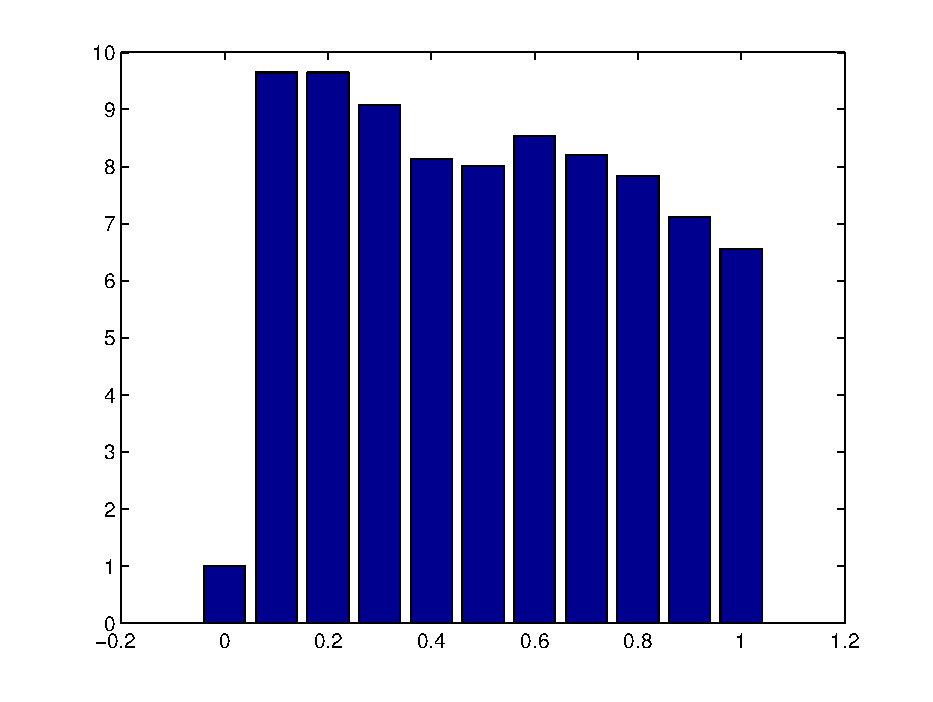
\includegraphics[scale=0.40]{images/tttExpectedGain}
	\caption{Mean gain after playing 100000 games of noughts and crosses with the given exploration rates.}
	\label{fig:tttExpectedGain}
\end{minipage}
\end{figure}

\section{Q-learning in BlackJack}

For Q-learning\cite{Sutton1998}, we retain the assumptions made in Section \ref{sec:td_ttt}.
However, the state structure will be a lookup table $Q$, instead of a tree.
$Q$ is a matrix of size $m \times n$, where $m$ is the number of states and $n$ is the number of actions.
Every time the agent takes an action $a_t$, the $Q$ value of the pair $\lbrace s_t, a_t \rbrace$ is updated as follows, $Q(s_t,a_t) = Q(s_t,a_t) + \alpha \left[ r_{t+1} + \gamma \max\limits_a Q(s_{t+1},a) - Q(s_t,a_t) \right]$, where $\alpha$ is the learning rate, $r_{t+1}$ is the reward for being in the state $s_{t+1}$ and $\gamma$ is a discounting factor.
An important advantage of using the aforementioned update mechanism, is its off-policy nature, since the $Q(s_t,a_t)$ will be updated with $\max\limits_a Q(s_{t+1},a)$, even if the policy chooses an action which is suboptimal, the update will be computed with the optimal $Q(s_{t+1},a)$ value.

Lets define the rules used for our blackjack implementation:

\begin{itemize}
  \item Cards are drawn from a 52 cards french deck.
  \item Cards points are the numeric value shown on the card, however kings, queens and jacks value is 10.
  \item The player may count one ace with 1 or 11 points.
  \item The player is dealt an initial two cards hand.
  \item The dealer must hit cards until they have 17 or more points.
  \item If the dealer and the player have the same number of points, the dealer wins.
\end{itemize}

With a reward of 10 for winning and -1 for loosing the mean gain for different exploration rates is shown in  Figure \ref{fig:blackjackExpectedGain}.
Since the dealer has an slight advantage, using equal rewards for winning and loosing produces negative expected gains, as shown in Figure \ref{fig:blackjackExpectedGain1}.
Policies learned after playing 100000 games are shown in Figures \ref{fig:blackjack_0_2_Q} and \ref{fig:blackjack_0_4_Q}.
With an ace in the hand, in both policies the agent stops hitting cards after their value is close to 18.
The agent plays more cautiously if it does not have any ace.
This policy makes sense since an ace can be counted as 11 points, so if the agent goes over 21 it can be recounted as 1 point.
Comparing both policies, we can see that with a higher exploration rate, the agent learnt that it should play even more prudently without an ace.

\begin{figure}[btph!]
\centering
\begin{minipage}[t]{0.45\linewidth}
	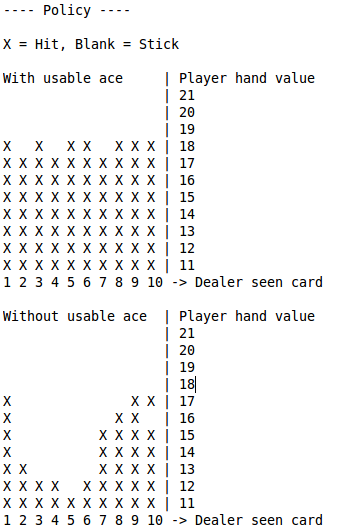
\includegraphics[scale=0.45]{images/blackjack_0_2_Q}
	\caption{Blackjack policy example, with 20\% exploration rate after 100000 games.}
	\label{fig:blackjack_0_2_Q}
\end{minipage}
\quad
\begin{minipage}[t]{0.45\linewidth}
	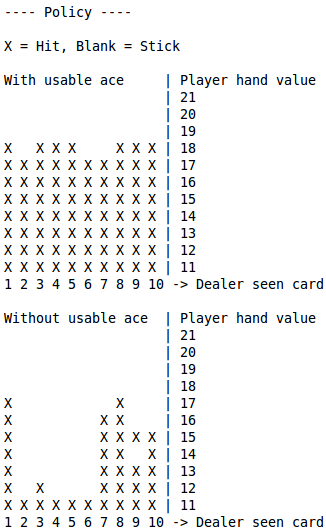
\includegraphics[scale=0.45]{images/blackjack_0_4_Q}
	\caption{Blackjack policy example, with 40\% exploration rate after 100000 games.}
	\label{fig:blackjack_0_4_Q}
\end{minipage}	

\end{figure}

\begin{figure}[htbp!]
\centering
\begin{minipage}[t]{0.45\linewidth}
	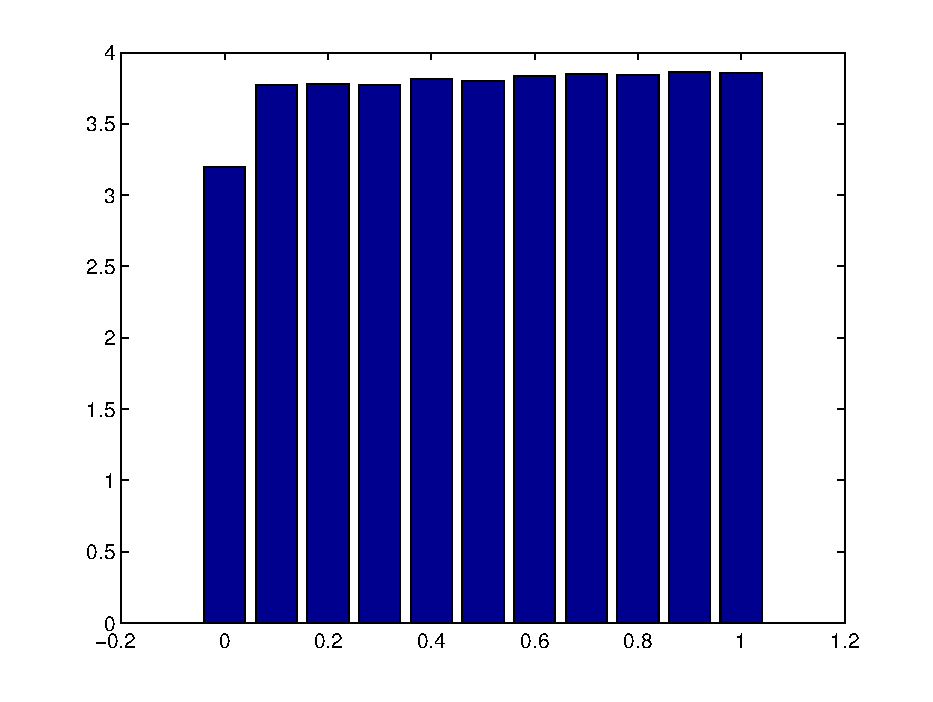
\includegraphics[scale=0.4]{images/blackjackExpectedGain2}
	\caption{Expected gain after playing 100000 games of blackjack with the given exploration rates.}
	\label{fig:blackjackExpectedGain}
\end{minipage}
\quad
\begin{minipage}[t]{0.45\linewidth}
	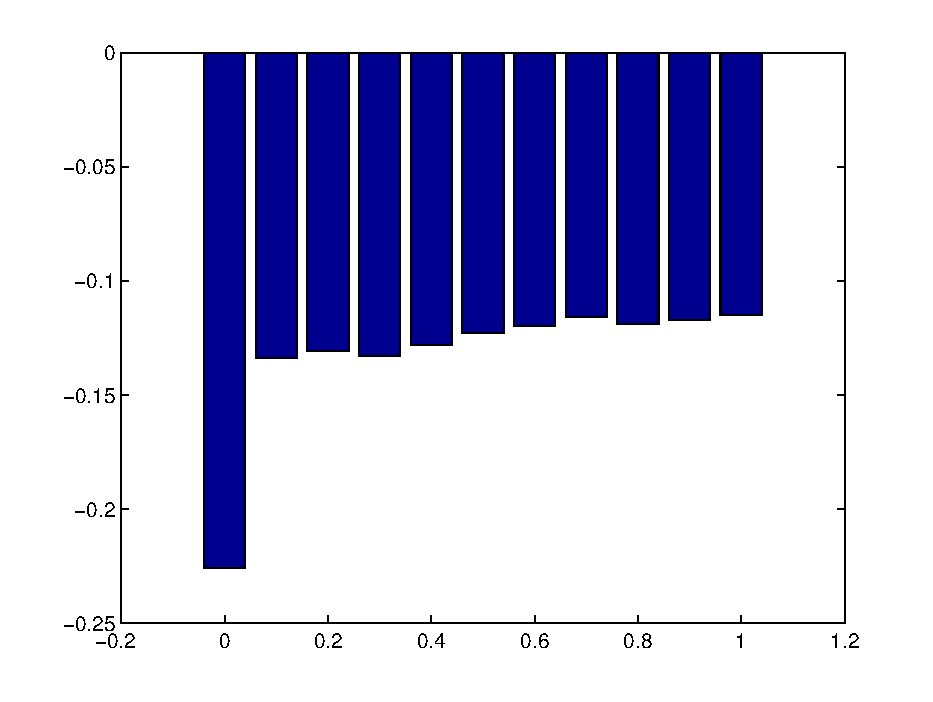
\includegraphics[scale=0.4]{images/blackjackExpectedGain1}
	\caption{Expected gain after playing 100000 games of blackjack with the given exploration rates.}
	\label{fig:blackjackExpectedGain1}
\end{minipage}	
\end{figure}

\section{Results and conclusions}

We have presented basic algorithms for path finding and reinforcement learning, which can be applied in games.
With A* we have a method that will output the optimal path, with minimal node evaluation for a given heuristic.
The heuristic distance could be overestimated in order to have a suboptimal path with early termination.
More advance path finding methods include D*\cite{Stentz1993} for incremental maps or Theta*\cite{Nash2007} for a continuous space map.
A substantial advantage of Q-learning, is its online learning component, therefore if implemented as the AI of the game, it can adapt to changes in the player strategy trough its continuous learning process.

\bibliographystyle{plain}
\bibliography{t3_report}

\end{document}

